% Add \usepackage{graphicx} in your preamble.
% Paths assume the manuscript is built from the repository root.
% These figures are designed at 7.16 inches; retain readable labels.
% For a two-column IEEE template, use figure* instead of figure.
\begin{figure}[t]
  \centering
  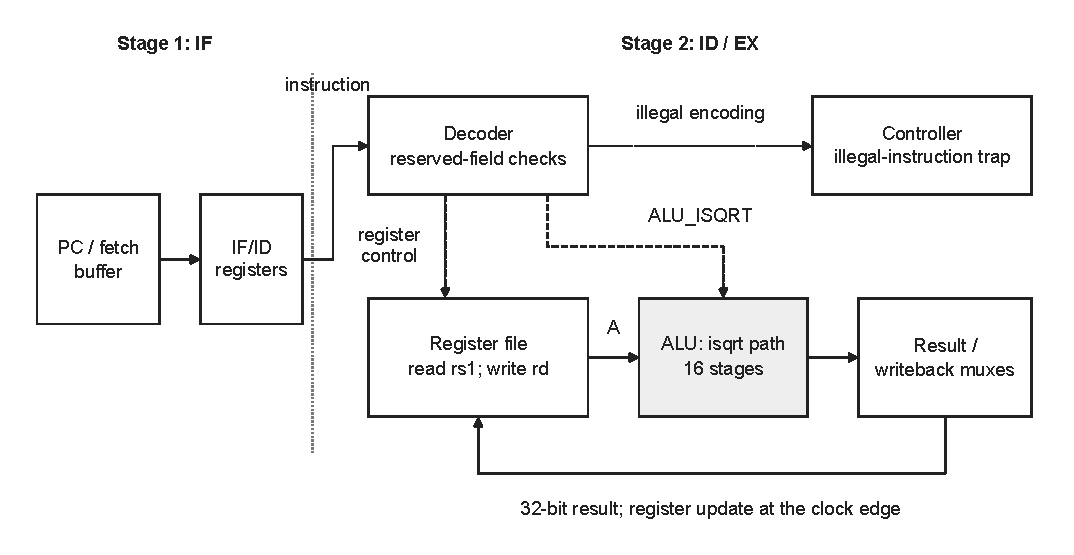
\includegraphics[width=\linewidth]{output/pdf/fig01_pipeline.pdf}
  \caption{Integration of the unsigned integer square-root instruction in the two-stage CVE2 pipeline. The shaded block denotes the added datapath within the existing ALU. The existing register-file write port captures the selected result at the closing clock edge. Dashed arrows denote control; solid arrows denote data. Only the relevant instruction and data paths are shown.}
  \label{fig:fig01_pipeline}
\end{figure}

\begin{figure}[t]
  \centering
  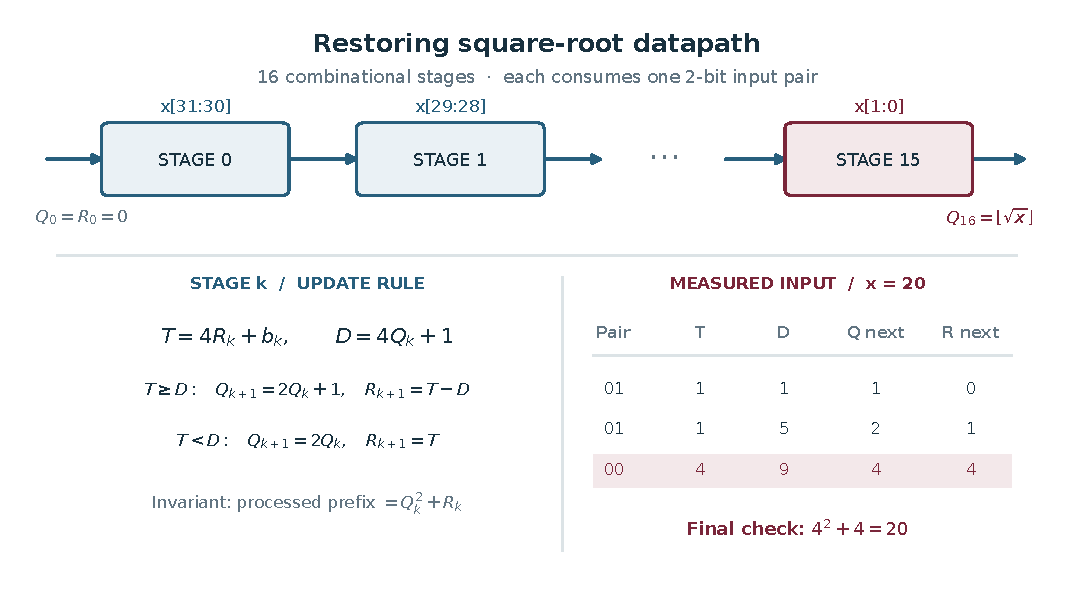
\includegraphics[width=\linewidth]{output/pdf/fig02_recurrence.pdf}
  \caption{Unrolled restoring square-root recurrence. Each stage consumes two input bits and produces one root bit. All 16 stages are combinational; there are no registers between stages. The worked example shows the final three stages for an input of 20; the preceding stages process zero pairs. The 16-bit root is zero-extended onto the 32-bit ALU result bus.}
  \label{fig:fig02_recurrence}
\end{figure}

\begin{figure}[t]
  \centering
  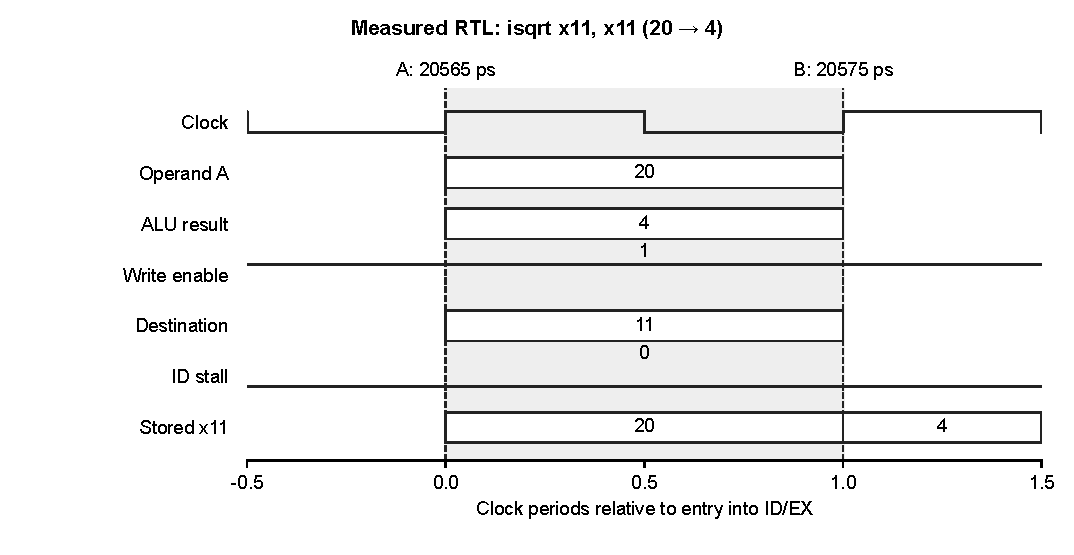
\includegraphics[width=\linewidth]{output/pdf/fig03_writeback.pdf}
  \caption{Sampled RTL waveform for isqrt a1, a1 with input 20. The register contains 20 during execution and updates to 4 at the next rising clock edge. The shaded interval has valid instruction and execution signals, no stall, and no illegal-instruction indication. Time is normalized to the observed clock period; the plot does not represent physical propagation delay. Operand, result and destination buses are shown only for the selected instruction.}
  \label{fig:fig03_writeback}
\end{figure}

